% chap4.tex (Definitions and Theorem)

\chapter{Model, Dataset, and Final Pipeline Description}
\section{Layer Descriptions}
\subsection{Embedding Layer}
An \textbf{embedding layer} maps an word index, or integer, into its corresponding embedding.
This layer is usually the first layer in a neural network that processes input such as text.
Given input text $s$, this layer receives as input a sequence of word indexes $BoW(\bm{s})=$ $\bm{x} = x_1,...,x_k$
and maps each word into an embedding.
Thus, for an input text $\bm{s}$, we transform it into a sequence of integers $\bm{x}$, and from there into $\mathbf{E} \in \mathbb{R}^{n \times d}$, where $d$ is
the embedding size. These embeddings are further fine-tuned during training. Because of the large number of
parameters in this layer (number of words allowed times embedding size), it is usually a good idea to
use $L_2$ regularization or dropout in order to avoid or mitigate overfitting.

\begin{figure}[H]
\caption{Visualization of an embedding layer. Word indexes are mapped to word embeddings. This
layer outputs a matrix comprised of stacked embeddings, one for each index.}
\centering
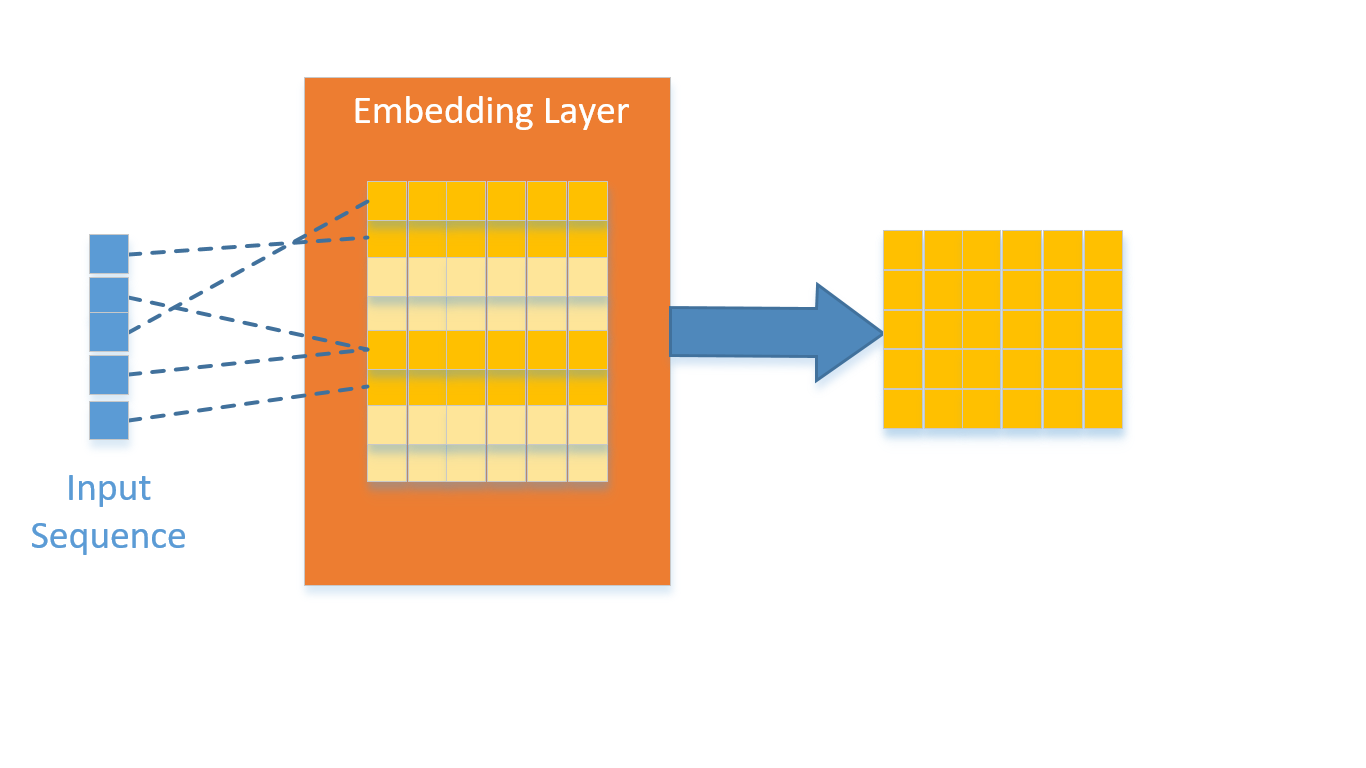
\includegraphics[width=0.5\textwidth]{EmbeddingLayer.png}
\end{figure}

\subsection{Feature Maps: Convolution + Pooling}

We refer to a convolutional layer followed by a pooling layer as a feature map.
Since our data are text sequences and thus have temporal structure, we use a one-dimensional convolutional
layer to convolve with embedding n-grams through the input sequence [CITE LANG AND HINTON 1988, WAIBEL ET AL 1989,
LANG ET AL 1990].
As in [REFER TO CONVOLUTION DIAGRAM], we stride only along the time dimension. This is in contrast to the usual two-dimensional convolution schemes with image data,
where the kernels stride along the width and height dimensions of the input data.
We use a global max pooling scheme to ouput a single value for each kernel[CITE LIN ET AL 2014]. Besides the huge
dimensionality reduction, we do this so that we pass to the next layer the single strongest activation
from each kernel i.e. a strong feature selection mechanism.

\subsection{Gated Recurrent Unit Layer}
A recurrent layer is designed to process data with temporal structure i.e. sequences [RUMELHART ET AL 1986].
This recurrent layer is in itself a network, where the hidden layer values at time \textit{t} depend on the previous
hidden layer's values, the input corresponding to time \textit{t}, and a shared parameter set:
\[\bm{h}^{t} = f(\bm{h}^{t-1}, \bm{x}^{t}, \bm{\theta})\]
This is implemented by \textit{unrolling} the layer along the time dimension as a sequence of layers, each corresponding
to the next in time. Because of this design, back propagation of error through the unrolled layer can result
in the vanishing gradient problem.

\begin{figure}[H]
\caption{Visualization of a recurrent layer. Each hidden layer $\bm{h}^{\textit{t}}$ is a function of the previous hidden
layer $\bm{h}^{\textit{t-1}}$, the present input signal $\bm{x}^{\textit{t}}$. The weights are shared across time steps
in order for the model to generalize better.}
\centering
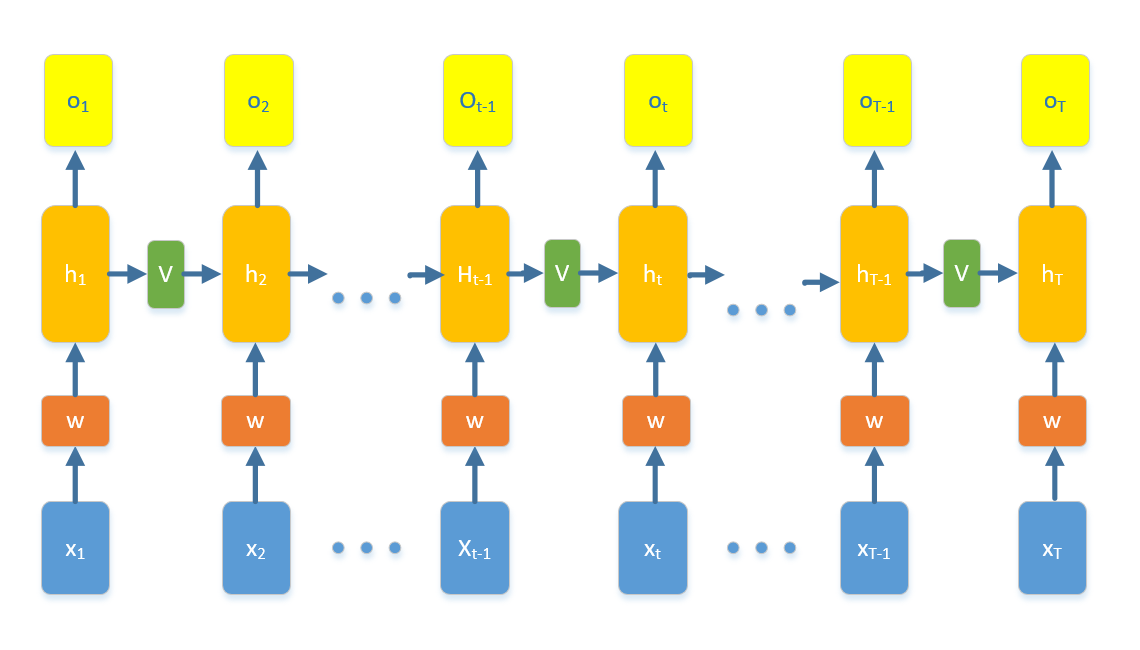
\includegraphics[width=0.5\textwidth]{RecurrentNet.png}
\end{figure}

A Gated Recurrent Unit layer is a type of recurrent layer designed to combat this condition[CITE CHO ET AL 2014].
It is a simplified version of the earlier LSTM layer[CITE SCHMIDHUBER], also designed to mitigate the vanishing gradient problem,
and in practice it performs comparably well.
This layer models the latent features computed by the feature map as a time sequence. This means that it
does not assume indepences between activation and learn to model the temporal structure of the previous
layer's output. This property makes the layer an adequate choice, since we deal with text data which inhibits
temporal structure.

\subsection{Dense Layer}
The last layer in our model is the classical \textbf{dense}, or fully connected layer.
The number of units in this layer is equal to the number of classes in our dataset.
Each unit $h_i$ is a linear combination of the previous layer's output with the unit's
corresponding set of weights. The \textbf{softmax} activation function is then applied to
the units, to finally output class probabilities.


\section{Model Description}

[YIN ET AL 2014] provide an overview of typical models used for text classification.
A standard architecture for convolutional neural networks for text sequence classification is the one proposed by
[CITE YOON 2014]. This model has an embedding layer followed by a feature map and a dense layer with a softmax activation
to output class probabilities.
Another popular neural model for text classification is the recurrent neural network. This model is
essentially an embedding layer followed by a recurrent layer e.g. LSTM or GRU, then a dense layer to output probabilities.
The model we use in this work is a mixture of these two standards: after the embedding layer, we add a feature map to learn the spatial
structure of the data, then we add a GRU layer. This design choice was made due to the fact that a recurrent layer
always led to better model performance, while the convolutional/pooling operations led to a huge data dimensionality reduction
and thus much faster training times. The two types of layers, combined, performed the best.


\begin{figure}[h]
\caption{Model Architecture: embedding layer, followed by two feature maps, and a recurrent layer. At the end, we have
a fully connected layer with a softmax activation, which will output class probabilities.}
\centering
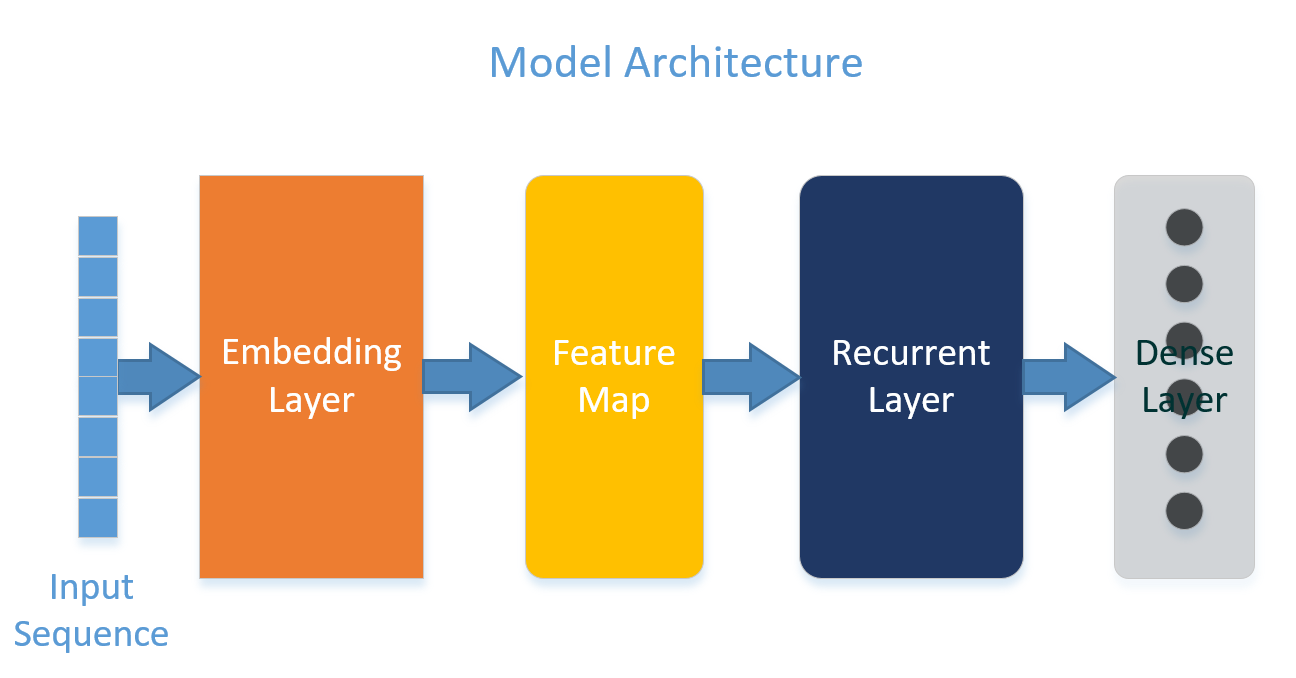
\includegraphics[width=0.5\textwidth]{ModelPipeline.png}
\end{figure}

Our network model is a variation of the convolutional model proposed by Yoon2014.
Our model consists of an embedding layer, two feature maps, a recurrent layer, and a dense layer.

The network's architecture is as follows:
\begin{itemize}
  \item Input layer: word index vector
  \item Embedding layer: maps word index vector to embedding matrix
  \item Feature Map 1:
      \begin{itemize}
        \item Convolution layer: number of kernels:32, activation: rectified linear
        \item MaxPooling layer
      \end{itemize}
\item Feature Map 2:
    \begin{itemize}
      \item Convolution layer: number of kernels:32, activation: rectified linear
      \item MaxPooling layer
    \end{itemize}
\item Gated Recurrent Unit layer
\item Dropout layer
\item Dense layer: output size: number of classes, activation: softmax
\end{itemize}

\section{Model Hyper-Parameters}
\begin{itemize}
  \item number of training words
  \item number of kernels
  \item kernel size
  \item pool size
  \item learning rate
  \item regularization rate
  \item dropout rate
  \item maximum sequence length

\end{itemize}

\section{Dataset Description}
[DESCRIBE AND CITE EMBEDDINGS]

We gathered scientific paper abstracts from the online repository Arxiv.org.
We scraped papers for 5 departments: computer science, mathematics, astrophysics, physics, quantitative biology, and quantititative finance.

\section{Final Pipeline}
[INCLUDE PIPELINE DIAGRAM]
